\documentclass[a4paper,12pt,twocolumn]{article}
%\usepackage[utf8x]{inputenc}
%\usepackage{CJK}
\usepackage[top=1in,bottom=1in,left=.8in,right=.8in]{geometry}
\usepackage{amsmath}
\usepackage{mathrsfs}
\usepackage{amssymb}
\usepackage{bm}
\usepackage{graphicx}
\usepackage{subfigure}
\usepackage{enumerate}
\usepackage{listings}
\lstset{language=C,breaklines,extendedchars=false,numbers=left}
% Title Page
%\begin{CJK}{UTF8}{gbsn}
\title{Position Based Fluid}
\author{Suyang Wang, Lei Yang and Beiling Lu \\Instructor: Ladislav Kavan\\Mentor:  Ishaan Singh}
\date{}



\begin{document}
\maketitle

\section{Introduction}
We implemented an interactive position based fluid simulation system that simulates fluid inside the Position Based Dynamics framework. The paper we are based on is the 2013 SIGGRAPH paper "Position Based Fluids" [Macklin et al. 2013]. In previous fluid simulation methods, such as the Smoothed Particle Hydrodynamics (SPH) method, enforcing incompressibility is crucial but computationally expensive, thus is impractical for real-time applications. This paper integrates the simulation process into the Position Based Dynamics (PBD) framework by solving a positional constraint that enforces constant density for each particle, and can achieve similar incompressibility and convergence to the SPH method but larger time steps that are suitable for real-time applications. In our project, we provides an interactive system implemented by following the algorithm in the paper. Also, we modified the collision detection method by applying constant position constraints on the static particles and depend fully on the PBD method for collision avoidance between the static particles and dynamic particles. The simulation system can be seen in the visual studio project, and several scenes captured in OpenGL and rendered in Maya can be found in the videos.


\section{Approach}
\subsection{Enforcing Incompressibility}
To enforce incompressibility of the water, we apply a position based constraint on each particle. First, following the principle of the SPH method, we calculate the density of each particle by applying a Poly6 kernel around its neighborhood, as shown in equation (\ref{densEst}).
\begin{equation}
\label{densEst}
\rho_i=\sum_j m_j W(\pmb p_i-\pmb p_j,h)
\end{equation}

As the standard approach in the position based dynamics, we solve a series of constraints to estimate the position of each particles of the fluid. The constrains is given by the form as equation(\ref{constraints}).
\begin{equation}
\label{constraints}
\pmb C_i(\pmb p_1,\cdots, \pmb p_n)=\cfrac{\rho_i}{\rho_0}-1
\end{equation}

where $\rho_0$ is the rest density specified by the property of the fluid.

based on the PBD method, we aim to find the position correction that satisfies the constraint in equation (\ref{pbdfunc})
\begin{equation}
\label{pbdfunc}
\pmb C(\pmb p+\Delta\pmb p)=0
\end{equation}

To achieve this, we first find the gradient of the constraint by looping through each particle in the scene, for each particle, we loop through itself and all of its neighbors, and apply the equation (\ref{gradspiky}) based on whether the particle is itself or its neighbor. In this step, we use the Spiky kernel.
\begin{equation}
\label{gradspiky}
\begin{split}
\nabla_{\pmb p_k}\pmb C_i=\cfrac{1}{\rho_0}\left\{
\begin{array}{lll}
\sum\limits_j \nabla_{\pmb p_k}W(\pmb p_i-\pmb p_j,h) &if\ k=i \\
\ &\ \\
-\nabla_{\pmb p_k}W(\pmb p_i-\pmb p_j,h) &if\ k=j
\end{array}
\right.
\end{split}
\end{equation}

Then we plug this gradient into the equation (\ref{lambda}) to compute the $\lambda$, where $\epsilon$ is the relaxation parameter.
\begin{equation}
\label{lambda}
\lambda_i=-\cfrac{\pmb C_i(\pmb p_1,\cdots,\pmb p_n)}{\sum_k\left|\nabla_{\pmb p_k}\pmb C_i\right|^2+\epsilon}
\end{equation}

With this equation, we can then deduce the position correction equation(\ref{pos}).
\begin{equation}
\label{pos}
\Delta {\pmb p_i}=\cfrac{1}{\rho_0}\sum_j(\lambda_i+\lambda_j)\nabla W(\pmb p_i-\pmb p_j,h)
\end{equation}

\subsection{Tensile Instability}
To prevent the problem of particle clustering or clumping caused by negative pressures when a particle has only a few neighbors and is unable to satisfy the rest density, we follow the paper's approach by adding an artificial pressure term (scorr) specified in terms of the smoothing kernel itself as in the equation (\ref{scorr}).
\begin{equation}
\label{scorr}
s_{corr}=-k\left(\cfrac{W(\pmb p_i-\pmb p_j,h)}{W(\Delta\pmb q,h)}\right)^n
\end{equation}

The position correction formula then becomes
\begin{equation}
\Delta {\pmb p_i}=\cfrac{1}{\rho_0}\sum_j(\lambda_i+\lambda_j+s_{corr})\nabla W(\pmb p_i-\pmb p_j,h)
\end{equation}


\subsection{Vorticity Confinement And Viscosity}
To compensate for additional damping caused by the nature of the PBD method, we use vorticity confinement to replace lost energy at each particle's location by using the estimator as in the equation (\ref{omega})
\begin{equation}
\label{omega}
\pmb\omega_i=\nabla \times \pmb v= \sum_j\pmb v_{ij} \times \nabla_{\pmb p_j}W(\pmb p_i-\pmb p_j,h)
\end{equation}

Then we calculate a corrective force using the equation (\ref{vorticity})
\begin{equation}
\label{vorticity}
\pmb f_i^{vorticity}=\epsilon(\pmb N \times \pmb\omega_i)
\end{equation}

where $\pmb N=\frac{\eta}{\|\eta\|}$ and $\eta=\Delta\|\pmb \omega\|_i$

In addition, we apply XSPH viscosity as in the equation (\ref{xsph}) to ensure coherent motion.
\begin{equation}
\label{xsph}
\pmb v_i^{new} = \pmb v_i+c\sum_j\pmb v_{ij}\cdot W(\pmb p_i-\pmb p_j,h)
\end{equation}
\subsection{Collision Detection}
\subsubsection{Boundary Collision Detection}
For the boundary condition, we used static collision detection scheme. As the global boundary, the configuration is set as a bounding box. The boundary constraint all the particles to be located in an limited spatial area, which enable us to use spatial grid to lower our complexity in neighbor finding which would be detailed descripted in the section Neighbor finding.
Simply detect the world coordinates of the particles, if one of the particles�� coordinates is out of the predefined region, the detector would reset its coordinate based on the collision position, velocity, and the surface normal.

\subsubsection{Collision with Object in the Scene}
Interactivity of fluid and obstacles is highly desired since this interactivity could introduce lots of interesting phenomenon. Traditionally, we would perform ray-triangulate intersection method to determine the collision. However, as the quantity of the particles in our scene, saying 4k to 10k, is extremely high, detecting collision of such scale would be totally out of our computational ability. To achieve real time collision detection ability, a number of methods could be applied. One way is to use Spatial Hash or Oct-tree method to decimate the quantity of potentially collision particles and triangles to test. But this methods still requires additional computation between the obstacles and the particles in the scene. What is more, the directional manipulate of the position and velocity of the fluid particles has large undesired side effects on the simulation which may result in the instable of the fluid. As we use the Position Based Dynamic scheme, we could simply employ the constant points constrains into our position based fluid scheme.
We treat the obstacles in the scene as the fluid particles. In this manner, we do not need to add any additional steps in finding potential collisions. All the obstacles points are set as constant points and they would not move in the scene. In previous section, we have discussed the density estimation. Since the obstacles are now only particles with constant position, they would have an additional influence when the neighbor particles estimate the density of itself. By adjusting the radius of the kernel and rest density, we could perform the real time collision detection with no additional tests. The only weakness of this method is that if the particle velocity is extremely high, this method might sometimes failed to correctly determine the collision. But these weakness could be easily avoided by limiting the scale of the scene and the time steps accordingly.
In our experiment, we have implemented several scenes to show our collision detection parts. In the Bunny container tests, we fill particles into the bunny and in the bottle of wine test, we perform collision detection between the bottle and the wine inside it.

\subsection{Neighbor Finding}
Neighbor finding has the complexity of $O(N^2)$ which would largely decrease the speed of our simulation. As the kernel function only affects particles inside its radius, we could boost up the neighbor finding process by dividing the space into grids.
We use a grid data structure which stores the pointer of the particles based on their spatial coordinates to speed up the neighbor finding process. The grid is divided based on the radius of the kernel function. Particles located in non-neighbor grids would never be neighbor particles, which means we only search neighbors in adjacent grid. In this manner, the time complexity of the neighbor finding is $O(N\cdot M^2)$, where $N$ is the time of particles costs by adding them to grid and $M$ is the number of particles in local grids. As the particles are relatively equally distributed in the space, the time costs by neighbor finding would decreased. There are cases in which most of the particles located in the same grid. We would limit the maximum number $M$ of neighbor particles to guarantee the efficiency of our approach.
\begin{figure*}[hbt]
  \centering
   \subfigure[Marching Cube]{
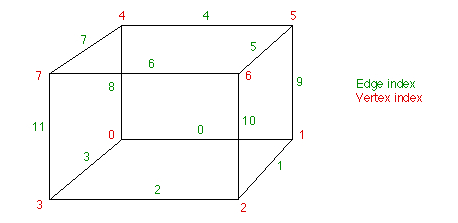
\includegraphics[width=.4\textwidth]{mcube1.png}
}
\subfigure[Surface Reconstruction]{
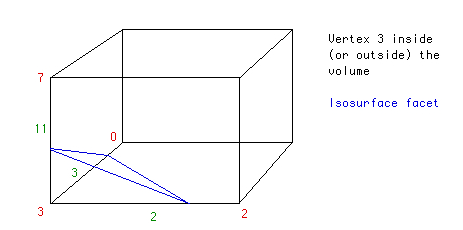
\includegraphics[width=.4\textwidth]{mcube2.png}
}
  % Requires \usepackage{graphicx}
 \caption{Marching Cube Algorithm}
 \label{mcube}
\end{figure*}

\subsection{Surface Reconstruction}
To construct surface for the fluid particles, we use Marching Cubes algorithm. The basic idea of the algorithm is to form a facet approximation to an isosurface through a scalar field sampled on a rectangular 3D grid. If one vertex is above the isosurface say and an adjacent vertex is below the isosurface then we know the isosurface cuts the edge between these two vertices. The position that it cuts the edge will be linearly interpolated, the ratio of the length between the two vertices will be the same as the ratio of the isosurface value to the values at the vertices of the grid cell.

The isosuface value we use here is the distance between each vertex on the marching cubes and particles in the grid. If the distance between the position of the corner of one cube and its closest particle in the surrounding grid is smaller than the threshold isovalue, then we can say this corner is below the surface.

The indexing convention for vertices and edges used in the algorithm are shown in figure(\ref{mcube}):


Then we use an edgeTable which maps the vertices under the isosurface to the intersecting edges to indicate each cube��s intersection information.  If $P_1$ and $P_2$ are the vertices of a cut edge and $V_1$ and $V_2$ are the scalar values at each vertex, the the intersection point P is given by \[P = P_1 + \cfrac{(isovalue - V_1) (P_2 - P_1) }{ (V_2 - V_1)}\]. By connecting each intersection points to be triangles, we can finally get a surface of current fluid particles.

\section{Challenges}
Firstly, in our implementation approach, we find some ambiguous detail when we go over the algorithm. As in equation (\ref{gradspiky}), we spend several hours in figuring out the relationships between the neighbor and the particle itself. We have tried both cases and find out the correct method to implement the task.

Secondly, as we use CPU to implement this originally GPU based method, the performance is an critical issue. Without the spatial grid in neighbor finding, the performance would be much worse than that now.

Third, we proposed a new scheme in collision detection by setting the obstacles as constant fluid particles in the scene. Using ray-triangle intersection would be an solution, but for a program with thousand particles, it is highly computational complex. We use this simple method to achieve well performance as well as nice collision handling result with no additional collision handling implemented. The scheme is fully compatible with the Position Based Dynamic scheme.

What is more, there are some more issues such as the gravity and the time step, iterations for density estimation. We searched the possibly parameters and choose them based on both performance and stability.
\section{Experiment Result}
\subsection{User Interactivity}
\begin{figure*}[!hbt]
  \centering
\subfigure[User interaction 1]{
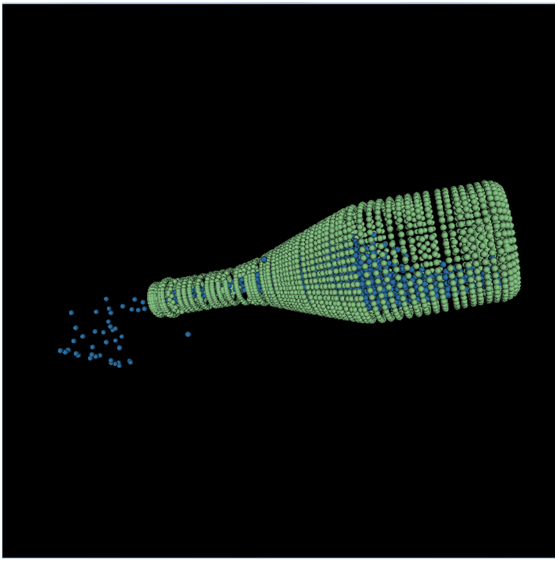
\includegraphics[width=.4\textwidth]{UserInteraction1.png}
}
\subfigure[User interaction 2]{
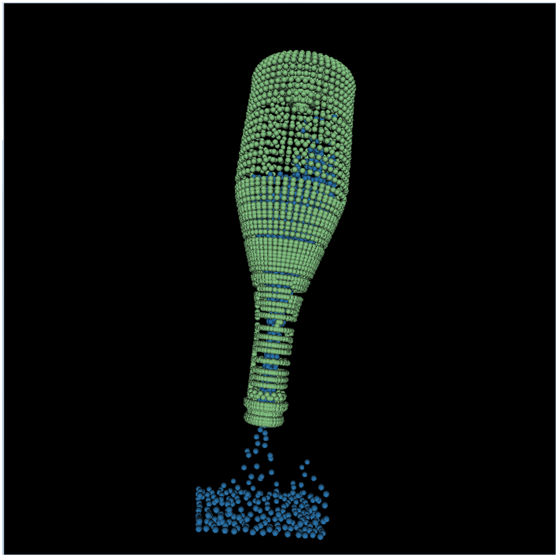
\includegraphics[width=.4\textwidth]{UserInteraction2.png}
}
  % Requires \usepackage{graphicx}
 \caption{User Interactivity}
 \label{mcube}
\end{figure*}
Our simulation system allows user to use mouse to control the rotation of the scene. By clicking and dragging the mouse, users can rotate the objects as well as the direction of the gravity force. Also, pressing 'g' or 'G' allows user to unlock the static particles, which will fall and become dynamic particles once they come into contact with the bounding box.

\subsection{Real-time Performance}
\begin{figure*}[!hbt]
  \centering
\subfigure[Bunny and funnel stay in the air]{
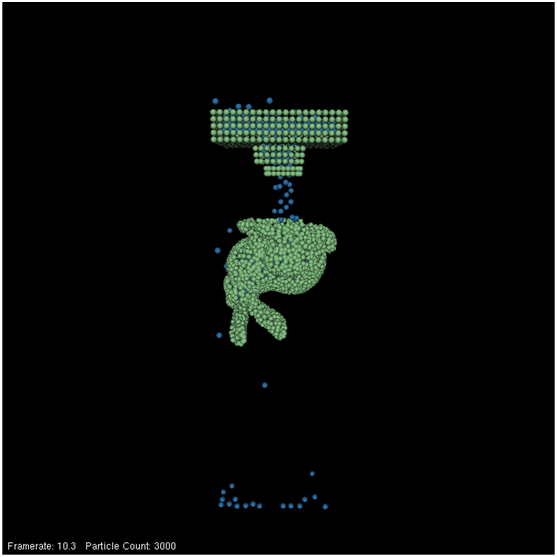
\includegraphics[width=.3\textwidth]{RealTime1.png}
}
\subfigure[After pressing 'g' bunny and funnel fall with gravity]{
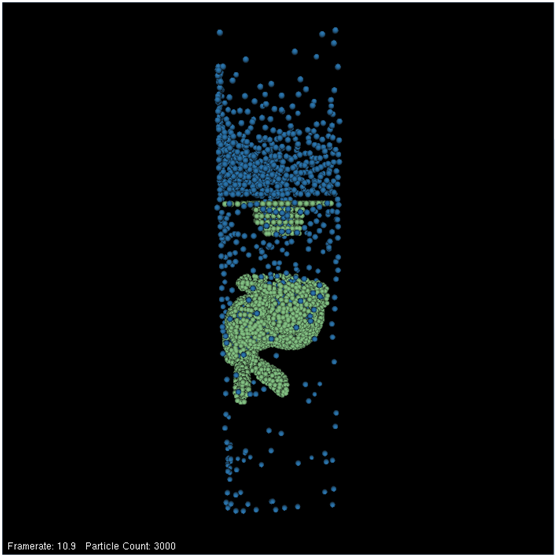
\includegraphics[width=.3\textwidth]{RealTime2.png}
}
\subfigure[Bunny and funnel merge into the dynamic particles]{
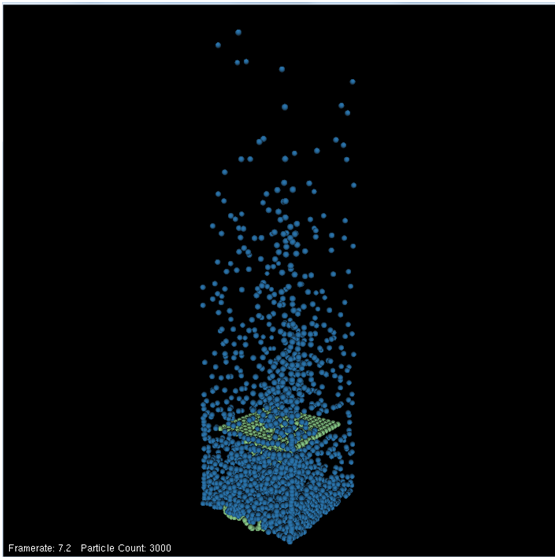
\includegraphics[width=.3\textwidth]{RealTime3.png}
}
  % Requires \usepackage{graphicx}
 \caption{Real Time performance}
 \label{mcube}
\end{figure*}
Our simulation system is based on CPU programming, and the typical number of particles it is able to support in order to provide real-time performance is 3K, with a FPS of approximately 10. The time step here is 0.05s, so the overall time costs for one second simulation is less than 1 second.

\subsection{OBJ File Loader}
\begin{figure*}[!hbt]
  \centering
\subfigure[Bunny and Funnel Container]{
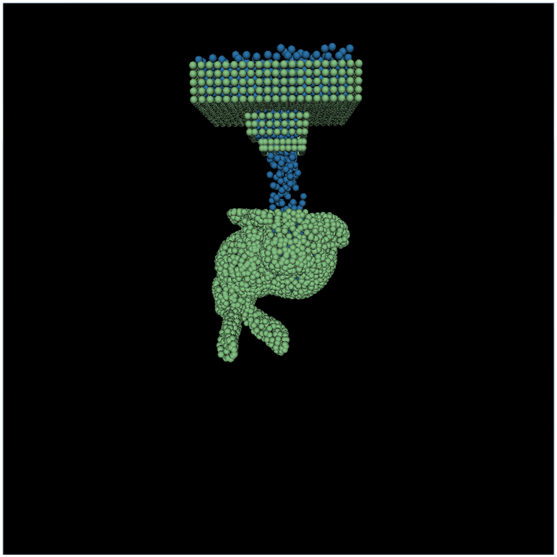
\includegraphics[width=.3\textwidth]{OBJ1.png}
}
\subfigure[Dragon Container]{
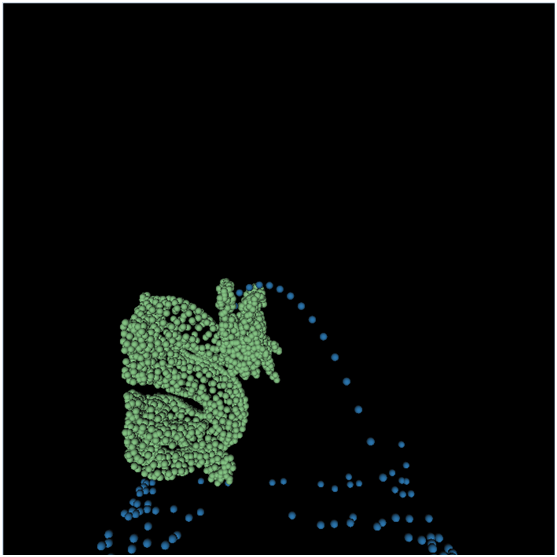
\includegraphics[width=.3\textwidth]{OBJ2.png}
}
\subfigure[Bottle Container]{
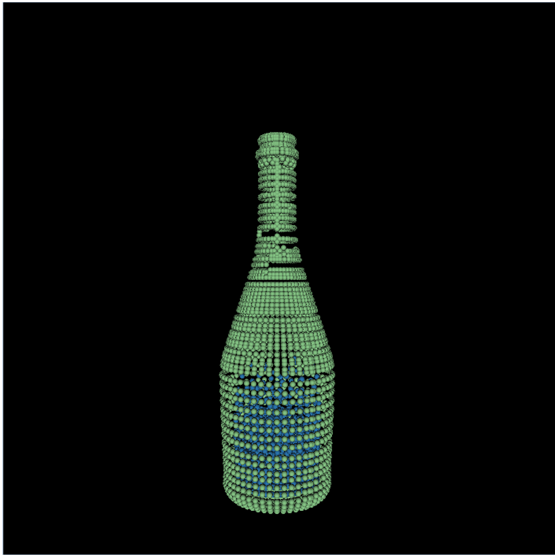
\includegraphics[width=.3\textwidth]{OBJ3.png}
}
  % Requires \usepackage{graphicx}
 \caption{Real Time performance}
 \label{mcube}
\end{figure*}
Our simulation system implemented an OBJ file loader to import multiple objects to define the shape of the container.

\subsection{Constant Points Constrains for Collision Detection}
For collision detection between the static particles and the dynamic particles, we makes use of the PBD method. By defining a larger rest density for the static particles and calculating the position correction for the dynamic particles in terms of the static particles, we ensure that the container made of static particles will hold the dynamic particles inside. For the collision detection between particles and the bounding box (not drawn in the scene), we still use geometric collision detection with the box.

\section{Different from related work}
We begin our project from the SPH procedure. The SPH requires 20 to 30 neighbors to estimate the pressure of a single particle, but with PBF, we do not need such large number of particles. In our implementation, even independent particle well followed the simulation process. Secondly, the time step of the PBF is much larger than the SPH method. It is more stable than SPH method.

What is more, we implemented the constant points constraints as our collision detection parts. This is different from all the previous works. We do not need to perform ray-triangle tests. The particle itself would exist pressures on the neighbor particles, which is as in the real world.
\section{Breakdown of Project}
\begin{itemize}
  \item Suyang and Beiling are focused on PBF implementation.
  \subitem Suyang implemented the basic data structure of the PBF solver and the algorithms. Suyang also implemented the OBJ loader parts.
  \subitem Beiling implemented the constant point constraints algorithm, interactive parts, visualization parts and program test.
  \item Lei is in charge of rendering and implemented the surface reconstruction part.
\end{itemize}

\begin{thebibliography}{99}
\bibitem{article1}Macklin, Miles, and Matthias M��ller. "Position based fluids." ACM Transactions on Graphics (TOG) 32, no. 4 (2013): 104.
\bibitem{article2}Bourke, Paul. "Polygonising a scalar field using tetrahedrons." (1997): 1-5.
\end{thebibliography}



%\end{CJK}
\end{document}

